
% Default to the notebook output style

    


% Inherit from the specified cell style.




    
\documentclass[11pt]{article}

    
    
    \usepackage[T1]{fontenc}
    % Nicer default font (+ math font) than Computer Modern for most use cases
    \usepackage{mathpazo}
	\usepackage{float}
    % Basic figure setup, for now with no caption control since it's done
    % automatically by Pandoc (which extracts ![](path) syntax from Markdown).
    \usepackage{graphicx}
    % We will generate all images so they have a width \maxwidth. This means
    % that they will get their normal width if they fit onto the page, but
    % are scaled down if they would overflow the margins.
    \makeatletter
    \def\maxwidth{\ifdim\Gin@nat@width>\linewidth\linewidth
    \else\Gin@nat@width\fi}
    \makeatother
    \let\Oldincludegraphics\includegraphics
    % Set max figure width to be 80% of text width, for now hardcoded.
    \renewcommand{\includegraphics}[1]{\Oldincludegraphics[width=.8\maxwidth]{#1}}
    % Ensure that by default, figures have no caption (until we provide a
    % proper Figure object with a Caption API and a way to capture that
    % in the conversion process - todo).
    \usepackage{caption}
    \DeclareCaptionLabelFormat{nolabel}{}
    \captionsetup{labelformat=nolabel}

    \usepackage{adjustbox} % Used to constrain images to a maximum size 
    \usepackage{xcolor} % Allow colors to be defined
    \usepackage{enumerate} % Needed for markdown enumerations to work
    \usepackage{geometry} % Used to adjust the document margins
    \usepackage{amsmath} % Equations
    \usepackage{amssymb} % Equations
    \usepackage{textcomp} % defines textquotesingle
    % Hack from http://tex.stackexchange.com/a/47451/13684:
    \AtBeginDocument{%
        \def\PYZsq{\textquotesingle}% Upright quotes in Pygmentized code
    }
    \usepackage{upquote} % Upright quotes for verbatim code
    \usepackage{eurosym} % defines \euro
    \usepackage[mathletters]{ucs} % Extended unicode (utf-8) support
    \usepackage[utf8x]{inputenc} % Allow utf-8 characters in the tex document
    \usepackage{fancyvrb} % verbatim replacement that allows latex
    \usepackage{grffile} % extends the file name processing of package graphics 
                         % to support a larger range 
    % The hyperref package gives us a pdf with properly built
    % internal navigation ('pdf bookmarks' for the table of contents,
    % internal cross-reference links, web links for URLs, etc.)
    \usepackage{hyperref}
    \usepackage{longtable} % longtable support required by pandoc >1.10
    \usepackage{booktabs}  % table support for pandoc > 1.12.2
    \usepackage[inline]{enumitem} % IRkernel/repr support (it uses the enumerate* environment)
    \usepackage[normalem]{ulem} % ulem is needed to support strikethroughs (\sout)
                                % normalem makes italics be italics, not underlines
    \usepackage{mathrsfs}
    

    
    
    % Colors for the hyperref package
    \definecolor{urlcolor}{rgb}{0,.145,.698}
    \definecolor{linkcolor}{rgb}{.71,0.21,0.01}
    \definecolor{citecolor}{rgb}{.12,.54,.11}

    % ANSI colors
    \definecolor{ansi-black}{HTML}{3E424D}
    \definecolor{ansi-black-intense}{HTML}{282C36}
    \definecolor{ansi-red}{HTML}{E75C58}
    \definecolor{ansi-red-intense}{HTML}{B22B31}
    \definecolor{ansi-green}{HTML}{00A250}
    \definecolor{ansi-green-intense}{HTML}{007427}
    \definecolor{ansi-yellow}{HTML}{DDB62B}
    \definecolor{ansi-yellow-intense}{HTML}{B27D12}
    \definecolor{ansi-blue}{HTML}{208FFB}
    \definecolor{ansi-blue-intense}{HTML}{0065CA}
    \definecolor{ansi-magenta}{HTML}{D160C4}
    \definecolor{ansi-magenta-intense}{HTML}{A03196}
    \definecolor{ansi-cyan}{HTML}{60C6C8}
    \definecolor{ansi-cyan-intense}{HTML}{258F8F}
    \definecolor{ansi-white}{HTML}{C5C1B4}
    \definecolor{ansi-white-intense}{HTML}{A1A6B2}
    \definecolor{ansi-default-inverse-fg}{HTML}{FFFFFF}
    \definecolor{ansi-default-inverse-bg}{HTML}{000000}

    % commands and environments needed by pandoc snippets
    % extracted from the output of `pandoc -s`
    \providecommand{\tightlist}{%
      \setlength{\itemsep}{0pt}\setlength{\parskip}{0pt}}
    \DefineVerbatimEnvironment{Highlighting}{Verbatim}{commandchars=\\\{\}}
    % Add ',fontsize=\small' for more characters per line
    \newenvironment{Shaded}{}{}
    \newcommand{\KeywordTok}[1]{\textcolor[rgb]{0.00,0.44,0.13}{\textbf{{#1}}}}
    \newcommand{\DataTypeTok}[1]{\textcolor[rgb]{0.56,0.13,0.00}{{#1}}}
    \newcommand{\DecValTok}[1]{\textcolor[rgb]{0.25,0.63,0.44}{{#1}}}
    \newcommand{\BaseNTok}[1]{\textcolor[rgb]{0.25,0.63,0.44}{{#1}}}
    \newcommand{\FloatTok}[1]{\textcolor[rgb]{0.25,0.63,0.44}{{#1}}}
    \newcommand{\CharTok}[1]{\textcolor[rgb]{0.25,0.44,0.63}{{#1}}}
    \newcommand{\StringTok}[1]{\textcolor[rgb]{0.25,0.44,0.63}{{#1}}}
    \newcommand{\CommentTok}[1]{\textcolor[rgb]{0.38,0.63,0.69}{\textit{{#1}}}}
    \newcommand{\OtherTok}[1]{\textcolor[rgb]{0.00,0.44,0.13}{{#1}}}
    \newcommand{\AlertTok}[1]{\textcolor[rgb]{1.00,0.00,0.00}{\textbf{{#1}}}}
    \newcommand{\FunctionTok}[1]{\textcolor[rgb]{0.02,0.16,0.49}{{#1}}}
    \newcommand{\RegionMarkerTok}[1]{{#1}}
    \newcommand{\ErrorTok}[1]{\textcolor[rgb]{1.00,0.00,0.00}{\textbf{{#1}}}}
    \newcommand{\NormalTok}[1]{{#1}}
    
    % Additional commands for more recent versions of Pandoc
    \newcommand{\ConstantTok}[1]{\textcolor[rgb]{0.53,0.00,0.00}{{#1}}}
    \newcommand{\SpecialCharTok}[1]{\textcolor[rgb]{0.25,0.44,0.63}{{#1}}}
    \newcommand{\VerbatimStringTok}[1]{\textcolor[rgb]{0.25,0.44,0.63}{{#1}}}
    \newcommand{\SpecialStringTok}[1]{\textcolor[rgb]{0.73,0.40,0.53}{{#1}}}
    \newcommand{\ImportTok}[1]{{#1}}
    \newcommand{\DocumentationTok}[1]{\textcolor[rgb]{0.73,0.13,0.13}{\textit{{#1}}}}
    \newcommand{\AnnotationTok}[1]{\textcolor[rgb]{0.38,0.63,0.69}{\textbf{\textit{{#1}}}}}
    \newcommand{\CommentVarTok}[1]{\textcolor[rgb]{0.38,0.63,0.69}{\textbf{\textit{{#1}}}}}
    \newcommand{\VariableTok}[1]{\textcolor[rgb]{0.10,0.09,0.49}{{#1}}}
    \newcommand{\ControlFlowTok}[1]{\textcolor[rgb]{0.00,0.44,0.13}{\textbf{{#1}}}}
    \newcommand{\OperatorTok}[1]{\textcolor[rgb]{0.40,0.40,0.40}{{#1}}}
    \newcommand{\BuiltInTok}[1]{{#1}}
    \newcommand{\ExtensionTok}[1]{{#1}}
    \newcommand{\PreprocessorTok}[1]{\textcolor[rgb]{0.74,0.48,0.00}{{#1}}}
    \newcommand{\AttributeTok}[1]{\textcolor[rgb]{0.49,0.56,0.16}{{#1}}}
    \newcommand{\InformationTok}[1]{\textcolor[rgb]{0.38,0.63,0.69}{\textbf{\textit{{#1}}}}}
    \newcommand{\WarningTok}[1]{\textcolor[rgb]{0.38,0.63,0.69}{\textbf{\textit{{#1}}}}}
    
    
    % Define a nice break command that doesn't care if a line doesn't already
    % exist.
    \def\br{\hspace*{\fill} \\* }
    % Math Jax compatibility definitions
    \def\gt{>}
    \def\lt{<}
    \let\Oldtex\TeX
    \let\Oldlatex\LaTeX
    \renewcommand{\TeX}{\textrm{\Oldtex}}
    \renewcommand{\LaTeX}{\textrm{\Oldlatex}}
    % Document parameters
    % Document title
    \title{Assignment 5}
    
    \author{Jiarong Ye}
    
    
    

    % Pygments definitions
    
\makeatletter
\def\PY@reset{\let\PY@it=\relax \let\PY@bf=\relax%
    \let\PY@ul=\relax \let\PY@tc=\relax%
    \let\PY@bc=\relax \let\PY@ff=\relax}
\def\PY@tok#1{\csname PY@tok@#1\endcsname}
\def\PY@toks#1+{\ifx\relax#1\empty\else%
    \PY@tok{#1}\expandafter\PY@toks\fi}
\def\PY@do#1{\PY@bc{\PY@tc{\PY@ul{%
    \PY@it{\PY@bf{\PY@ff{#1}}}}}}}
\def\PY#1#2{\PY@reset\PY@toks#1+\relax+\PY@do{#2}}

\expandafter\def\csname PY@tok@w\endcsname{\def\PY@tc##1{\textcolor[rgb]{0.73,0.73,0.73}{##1}}}
\expandafter\def\csname PY@tok@c\endcsname{\let\PY@it=\textit\def\PY@tc##1{\textcolor[rgb]{0.25,0.50,0.50}{##1}}}
\expandafter\def\csname PY@tok@cp\endcsname{\def\PY@tc##1{\textcolor[rgb]{0.74,0.48,0.00}{##1}}}
\expandafter\def\csname PY@tok@k\endcsname{\let\PY@bf=\textbf\def\PY@tc##1{\textcolor[rgb]{0.00,0.50,0.00}{##1}}}
\expandafter\def\csname PY@tok@kp\endcsname{\def\PY@tc##1{\textcolor[rgb]{0.00,0.50,0.00}{##1}}}
\expandafter\def\csname PY@tok@kt\endcsname{\def\PY@tc##1{\textcolor[rgb]{0.69,0.00,0.25}{##1}}}
\expandafter\def\csname PY@tok@o\endcsname{\def\PY@tc##1{\textcolor[rgb]{0.40,0.40,0.40}{##1}}}
\expandafter\def\csname PY@tok@ow\endcsname{\let\PY@bf=\textbf\def\PY@tc##1{\textcolor[rgb]{0.67,0.13,1.00}{##1}}}
\expandafter\def\csname PY@tok@nb\endcsname{\def\PY@tc##1{\textcolor[rgb]{0.00,0.50,0.00}{##1}}}
\expandafter\def\csname PY@tok@nf\endcsname{\def\PY@tc##1{\textcolor[rgb]{0.00,0.00,1.00}{##1}}}
\expandafter\def\csname PY@tok@nc\endcsname{\let\PY@bf=\textbf\def\PY@tc##1{\textcolor[rgb]{0.00,0.00,1.00}{##1}}}
\expandafter\def\csname PY@tok@nn\endcsname{\let\PY@bf=\textbf\def\PY@tc##1{\textcolor[rgb]{0.00,0.00,1.00}{##1}}}
\expandafter\def\csname PY@tok@ne\endcsname{\let\PY@bf=\textbf\def\PY@tc##1{\textcolor[rgb]{0.82,0.25,0.23}{##1}}}
\expandafter\def\csname PY@tok@nv\endcsname{\def\PY@tc##1{\textcolor[rgb]{0.10,0.09,0.49}{##1}}}
\expandafter\def\csname PY@tok@no\endcsname{\def\PY@tc##1{\textcolor[rgb]{0.53,0.00,0.00}{##1}}}
\expandafter\def\csname PY@tok@nl\endcsname{\def\PY@tc##1{\textcolor[rgb]{0.63,0.63,0.00}{##1}}}
\expandafter\def\csname PY@tok@ni\endcsname{\let\PY@bf=\textbf\def\PY@tc##1{\textcolor[rgb]{0.60,0.60,0.60}{##1}}}
\expandafter\def\csname PY@tok@na\endcsname{\def\PY@tc##1{\textcolor[rgb]{0.49,0.56,0.16}{##1}}}
\expandafter\def\csname PY@tok@nt\endcsname{\let\PY@bf=\textbf\def\PY@tc##1{\textcolor[rgb]{0.00,0.50,0.00}{##1}}}
\expandafter\def\csname PY@tok@nd\endcsname{\def\PY@tc##1{\textcolor[rgb]{0.67,0.13,1.00}{##1}}}
\expandafter\def\csname PY@tok@s\endcsname{\def\PY@tc##1{\textcolor[rgb]{0.73,0.13,0.13}{##1}}}
\expandafter\def\csname PY@tok@sd\endcsname{\let\PY@it=\textit\def\PY@tc##1{\textcolor[rgb]{0.73,0.13,0.13}{##1}}}
\expandafter\def\csname PY@tok@si\endcsname{\let\PY@bf=\textbf\def\PY@tc##1{\textcolor[rgb]{0.73,0.40,0.53}{##1}}}
\expandafter\def\csname PY@tok@se\endcsname{\let\PY@bf=\textbf\def\PY@tc##1{\textcolor[rgb]{0.73,0.40,0.13}{##1}}}
\expandafter\def\csname PY@tok@sr\endcsname{\def\PY@tc##1{\textcolor[rgb]{0.73,0.40,0.53}{##1}}}
\expandafter\def\csname PY@tok@ss\endcsname{\def\PY@tc##1{\textcolor[rgb]{0.10,0.09,0.49}{##1}}}
\expandafter\def\csname PY@tok@sx\endcsname{\def\PY@tc##1{\textcolor[rgb]{0.00,0.50,0.00}{##1}}}
\expandafter\def\csname PY@tok@m\endcsname{\def\PY@tc##1{\textcolor[rgb]{0.40,0.40,0.40}{##1}}}
\expandafter\def\csname PY@tok@gh\endcsname{\let\PY@bf=\textbf\def\PY@tc##1{\textcolor[rgb]{0.00,0.00,0.50}{##1}}}
\expandafter\def\csname PY@tok@gu\endcsname{\let\PY@bf=\textbf\def\PY@tc##1{\textcolor[rgb]{0.50,0.00,0.50}{##1}}}
\expandafter\def\csname PY@tok@gd\endcsname{\def\PY@tc##1{\textcolor[rgb]{0.63,0.00,0.00}{##1}}}
\expandafter\def\csname PY@tok@gi\endcsname{\def\PY@tc##1{\textcolor[rgb]{0.00,0.63,0.00}{##1}}}
\expandafter\def\csname PY@tok@gr\endcsname{\def\PY@tc##1{\textcolor[rgb]{1.00,0.00,0.00}{##1}}}
\expandafter\def\csname PY@tok@ge\endcsname{\let\PY@it=\textit}
\expandafter\def\csname PY@tok@gs\endcsname{\let\PY@bf=\textbf}
\expandafter\def\csname PY@tok@gp\endcsname{\let\PY@bf=\textbf\def\PY@tc##1{\textcolor[rgb]{0.00,0.00,0.50}{##1}}}
\expandafter\def\csname PY@tok@go\endcsname{\def\PY@tc##1{\textcolor[rgb]{0.53,0.53,0.53}{##1}}}
\expandafter\def\csname PY@tok@gt\endcsname{\def\PY@tc##1{\textcolor[rgb]{0.00,0.27,0.87}{##1}}}
\expandafter\def\csname PY@tok@err\endcsname{\def\PY@bc##1{\setlength{\fboxsep}{0pt}\fcolorbox[rgb]{1.00,0.00,0.00}{1,1,1}{\strut ##1}}}
\expandafter\def\csname PY@tok@kc\endcsname{\let\PY@bf=\textbf\def\PY@tc##1{\textcolor[rgb]{0.00,0.50,0.00}{##1}}}
\expandafter\def\csname PY@tok@kd\endcsname{\let\PY@bf=\textbf\def\PY@tc##1{\textcolor[rgb]{0.00,0.50,0.00}{##1}}}
\expandafter\def\csname PY@tok@kn\endcsname{\let\PY@bf=\textbf\def\PY@tc##1{\textcolor[rgb]{0.00,0.50,0.00}{##1}}}
\expandafter\def\csname PY@tok@kr\endcsname{\let\PY@bf=\textbf\def\PY@tc##1{\textcolor[rgb]{0.00,0.50,0.00}{##1}}}
\expandafter\def\csname PY@tok@bp\endcsname{\def\PY@tc##1{\textcolor[rgb]{0.00,0.50,0.00}{##1}}}
\expandafter\def\csname PY@tok@fm\endcsname{\def\PY@tc##1{\textcolor[rgb]{0.00,0.00,1.00}{##1}}}
\expandafter\def\csname PY@tok@vc\endcsname{\def\PY@tc##1{\textcolor[rgb]{0.10,0.09,0.49}{##1}}}
\expandafter\def\csname PY@tok@vg\endcsname{\def\PY@tc##1{\textcolor[rgb]{0.10,0.09,0.49}{##1}}}
\expandafter\def\csname PY@tok@vi\endcsname{\def\PY@tc##1{\textcolor[rgb]{0.10,0.09,0.49}{##1}}}
\expandafter\def\csname PY@tok@vm\endcsname{\def\PY@tc##1{\textcolor[rgb]{0.10,0.09,0.49}{##1}}}
\expandafter\def\csname PY@tok@sa\endcsname{\def\PY@tc##1{\textcolor[rgb]{0.73,0.13,0.13}{##1}}}
\expandafter\def\csname PY@tok@sb\endcsname{\def\PY@tc##1{\textcolor[rgb]{0.73,0.13,0.13}{##1}}}
\expandafter\def\csname PY@tok@sc\endcsname{\def\PY@tc##1{\textcolor[rgb]{0.73,0.13,0.13}{##1}}}
\expandafter\def\csname PY@tok@dl\endcsname{\def\PY@tc##1{\textcolor[rgb]{0.73,0.13,0.13}{##1}}}
\expandafter\def\csname PY@tok@s2\endcsname{\def\PY@tc##1{\textcolor[rgb]{0.73,0.13,0.13}{##1}}}
\expandafter\def\csname PY@tok@sh\endcsname{\def\PY@tc##1{\textcolor[rgb]{0.73,0.13,0.13}{##1}}}
\expandafter\def\csname PY@tok@s1\endcsname{\def\PY@tc##1{\textcolor[rgb]{0.73,0.13,0.13}{##1}}}
\expandafter\def\csname PY@tok@mb\endcsname{\def\PY@tc##1{\textcolor[rgb]{0.40,0.40,0.40}{##1}}}
\expandafter\def\csname PY@tok@mf\endcsname{\def\PY@tc##1{\textcolor[rgb]{0.40,0.40,0.40}{##1}}}
\expandafter\def\csname PY@tok@mh\endcsname{\def\PY@tc##1{\textcolor[rgb]{0.40,0.40,0.40}{##1}}}
\expandafter\def\csname PY@tok@mi\endcsname{\def\PY@tc##1{\textcolor[rgb]{0.40,0.40,0.40}{##1}}}
\expandafter\def\csname PY@tok@il\endcsname{\def\PY@tc##1{\textcolor[rgb]{0.40,0.40,0.40}{##1}}}
\expandafter\def\csname PY@tok@mo\endcsname{\def\PY@tc##1{\textcolor[rgb]{0.40,0.40,0.40}{##1}}}
\expandafter\def\csname PY@tok@ch\endcsname{\let\PY@it=\textit\def\PY@tc##1{\textcolor[rgb]{0.25,0.50,0.50}{##1}}}
\expandafter\def\csname PY@tok@cm\endcsname{\let\PY@it=\textit\def\PY@tc##1{\textcolor[rgb]{0.25,0.50,0.50}{##1}}}
\expandafter\def\csname PY@tok@cpf\endcsname{\let\PY@it=\textit\def\PY@tc##1{\textcolor[rgb]{0.25,0.50,0.50}{##1}}}
\expandafter\def\csname PY@tok@c1\endcsname{\let\PY@it=\textit\def\PY@tc##1{\textcolor[rgb]{0.25,0.50,0.50}{##1}}}
\expandafter\def\csname PY@tok@cs\endcsname{\let\PY@it=\textit\def\PY@tc##1{\textcolor[rgb]{0.25,0.50,0.50}{##1}}}

\def\PYZbs{\char`\\}
\def\PYZus{\char`\_}
\def\PYZob{\char`\{}
\def\PYZcb{\char`\}}
\def\PYZca{\char`\^}
\def\PYZam{\char`\&}
\def\PYZlt{\char`\<}
\def\PYZgt{\char`\>}
\def\PYZsh{\char`\#}
\def\PYZpc{\char`\%}
\def\PYZdl{\char`\$}
\def\PYZhy{\char`\-}
\def\PYZsq{\char`\'}
\def\PYZdq{\char`\"}
\def\PYZti{\char`\~}
% for compatibility with earlier versions
\def\PYZat{@}
\def\PYZlb{[}
\def\PYZrb{]}
\makeatother


    % Exact colors from NB
    \definecolor{incolor}{rgb}{0.0, 0.0, 0.5}
    \definecolor{outcolor}{rgb}{0.545, 0.0, 0.0}



    
    % Prevent overflowing lines due to hard-to-break entities
    \sloppy 
    % Setup hyperref package
    \hypersetup{
      breaklinks=true,  % so long urls are correctly broken across lines
      colorlinks=true,
      urlcolor=urlcolor,
      linkcolor=linkcolor,
      citecolor=citecolor,
      }
    % Slightly bigger margins than the latex defaults
    
    \geometry{verbose,tmargin=1in,bmargin=1in,lmargin=1in,rmargin=1in}
    
    

    \begin{document}
    
    
    \maketitle
    
    

    
    \subsection*{Q1}\label{q1}

\begin{enumerate}
\def\labelenumi{\arabic{enumi}.}
\tightlist
\item
  (30\%) Perform K-means on the data shown in Table 1. Use K=2 and
  suppose A and C are randomly selected as initial means. Please show
  the clustering results of nodes of each round until converged.
\end{enumerate}

\begin{figure}[H]
\centering
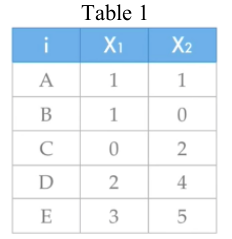
\includegraphics{1.png}
\caption{}
\end{figure}

    \begin{Verbatim}[commandchars=\\\{\}]
{\color{incolor}In [{\color{incolor}43}]:} \PY{c+c1}{\PYZsh{} slightly adjust the programming assignment }
         
         \PY{k+kn}{import} \PY{n+nn}{numpy} \PY{k}{as} \PY{n+nn}{np}
         \PY{k+kn}{from} \PY{n+nn}{collections} \PY{k}{import} \PY{n}{Counter}
         \PY{k+kn}{import} \PY{n+nn}{matplotlib}\PY{n+nn}{.}\PY{n+nn}{pyplot} \PY{k}{as} \PY{n+nn}{plt}
         \PY{k+kn}{from} \PY{n+nn}{sklearn}\PY{n+nn}{.}\PY{n+nn}{metrics} \PY{k}{import} \PY{n}{f1\PYZus{}score}\PY{p}{,} \PY{n}{normalized\PYZus{}mutual\PYZus{}info\PYZus{}score}
         
         \PY{n}{THRESHOLD} \PY{o}{=} \PY{l+m+mf}{1e\PYZhy{}5}
         
         \PY{n}{X} \PY{o}{=} \PY{n}{np}\PY{o}{.}\PY{n}{array}\PY{p}{(}\PY{p}{[}\PY{p}{[}\PY{l+m+mi}{1}\PY{p}{,}\PY{l+m+mi}{1}\PY{p}{]}\PY{p}{,}
                       \PY{p}{[}\PY{l+m+mi}{1}\PY{p}{,}\PY{l+m+mi}{0}\PY{p}{]}\PY{p}{,}
                       \PY{p}{[}\PY{l+m+mi}{0}\PY{p}{,}\PY{l+m+mi}{2}\PY{p}{]}\PY{p}{,}
                       \PY{p}{[}\PY{l+m+mi}{2}\PY{p}{,}\PY{l+m+mi}{4}\PY{p}{]}\PY{p}{,}
                       \PY{p}{[}\PY{l+m+mi}{3}\PY{p}{,}\PY{l+m+mi}{5}\PY{p}{]}\PY{p}{]}\PY{p}{)}
         
         \PY{k}{def} \PY{n+nf}{norm}\PY{p}{(}\PY{n}{x}\PY{p}{)}\PY{p}{:}
             \PY{n}{max\PYZus{}val} \PY{o}{=} \PY{n}{np}\PY{o}{.}\PY{n}{max}\PY{p}{(}\PY{n}{x}\PY{p}{,} \PY{n}{axis}\PY{o}{=}\PY{l+m+mi}{0}\PY{p}{)}
             \PY{n}{x} \PY{o}{=} \PY{n}{x} \PY{o}{/} \PY{n}{max\PYZus{}val}
             \PY{k}{return} \PY{n}{x}
         
         \PY{k}{def} \PY{n+nf}{converged}\PY{p}{(}\PY{n}{centroids1}\PY{p}{,} \PY{n}{centroids2}\PY{p}{)}\PY{p}{:}
             \PY{n}{diff} \PY{o}{=} \PY{n}{np}\PY{o}{.}\PY{n}{sum}\PY{p}{(}\PY{n}{np}\PY{o}{.}\PY{n}{abs}\PY{p}{(}\PY{n}{np}\PY{o}{.}\PY{n}{sum}\PY{p}{(}\PY{n}{centroids1} \PY{o}{\PYZhy{}} \PY{n}{centroids2}\PY{p}{,} \PY{n}{axis}\PY{o}{=}\PY{l+m+mi}{1}\PY{p}{)}\PY{p}{)}\PY{p}{,} \PY{n}{axis}\PY{o}{=}\PY{l+m+mi}{0}\PY{p}{)}
             \PY{k}{if} \PY{n}{np}\PY{o}{.}\PY{n}{equal}\PY{p}{(}\PY{n}{centroids1}\PY{p}{,} \PY{n}{centroids2}\PY{p}{)}\PY{o}{.}\PY{n}{all}\PY{p}{(}\PY{p}{)}\PY{p}{:}
                 \PY{k}{return} \PY{k+kc}{True}
             \PY{k}{elif} \PY{n}{diff} \PY{o}{\PYZlt{}} \PY{n}{THRESHOLD}\PY{p}{:}
                 \PY{k}{return} \PY{k+kc}{True}
             \PY{k}{else}\PY{p}{:}
                 \PY{k}{return} \PY{k+kc}{False}
         
         \PY{k}{def} \PY{n+nf}{euclidean\PYZus{}dist}\PY{p}{(}\PY{n}{x1}\PY{p}{,} \PY{n}{x2}\PY{p}{)}\PY{p}{:}
             \PY{k}{return} \PY{n}{np}\PY{o}{.}\PY{n}{sqrt}\PY{p}{(}\PY{n}{np}\PY{o}{.}\PY{n}{sum}\PY{p}{(}\PY{n}{np}\PY{o}{.}\PY{n}{square}\PY{p}{(}\PY{n}{x1} \PY{o}{\PYZhy{}} \PY{n}{x2}\PY{p}{)}\PY{p}{,} \PY{n}{axis}\PY{o}{=}\PY{l+m+mi}{1}\PY{p}{)}\PY{p}{)}
         
         
         \PY{k}{def} \PY{n+nf}{closest\PYZus{}centroid}\PY{p}{(}\PY{n}{val}\PY{p}{,} \PY{n}{centroids}\PY{p}{)}\PY{p}{:}
             \PY{k}{return} \PY{n}{np}\PY{o}{.}\PY{n}{argmin}\PY{p}{(}\PY{n}{np}\PY{o}{.}\PY{n}{sqrt}\PY{p}{(}\PY{n}{np}\PY{o}{.}\PY{n}{sum}\PY{p}{(}\PY{n}{np}\PY{o}{.}\PY{n}{square}\PY{p}{(}\PY{n}{val} \PY{o}{\PYZhy{}} \PY{n}{centroids}\PY{p}{)}\PY{p}{,} \PY{n}{axis}\PY{o}{=}\PY{l+m+mi}{1}\PY{p}{)}\PY{p}{)}\PY{p}{)}
         
         
         \PY{k}{def} \PY{n+nf}{update\PYZus{}centroids}\PY{p}{(}\PY{n}{data}\PY{p}{,} \PY{n}{centroids}\PY{p}{,} \PY{n}{k}\PY{o}{=}\PY{l+m+mi}{2}\PY{p}{)}\PY{p}{:}
             \PY{n}{n\PYZus{}samples} \PY{o}{=} \PY{n}{np}\PY{o}{.}\PY{n}{shape}\PY{p}{(}\PY{n}{data}\PY{p}{)}\PY{p}{[}\PY{l+m+mi}{0}\PY{p}{]}
             \PY{n}{n\PYZus{}features} \PY{o}{=} \PY{n}{np}\PY{o}{.}\PY{n}{shape}\PY{p}{(}\PY{n}{data}\PY{p}{)}\PY{p}{[}\PY{l+m+mi}{1}\PY{p}{]}
             \PY{n}{clusters} \PY{o}{=} \PY{p}{[}\PY{p}{[}\PY{p}{]} \PY{k}{for} \PY{n}{\PYZus{}} \PY{o+ow}{in} \PY{n+nb}{range}\PY{p}{(}\PY{n}{k}\PY{p}{)}\PY{p}{]}
             \PY{n}{labels} \PY{o}{=} \PY{n}{np}\PY{o}{.}\PY{n}{zeros}\PY{p}{(}\PY{p}{(}\PY{n}{n\PYZus{}samples}\PY{p}{)}\PY{p}{)}
         
             \PY{k}{for} \PY{n}{idx}\PY{p}{,} \PY{n}{val} \PY{o+ow}{in} \PY{n+nb}{enumerate}\PY{p}{(}\PY{n}{data}\PY{p}{)}\PY{p}{:}
                 \PY{n}{val\PYZus{}label} \PY{o}{=} \PY{n}{closest\PYZus{}centroid}\PY{p}{(}\PY{n}{val}\PY{p}{,} \PY{n}{centroids}\PY{p}{)}
                 \PY{n}{clusters}\PY{p}{[}\PY{n}{val\PYZus{}label}\PY{p}{]}\PY{o}{.}\PY{n}{append}\PY{p}{(}\PY{n}{val}\PY{p}{)}
                 \PY{n}{labels}\PY{p}{[}\PY{n}{idx}\PY{p}{]} \PY{o}{=} \PY{n}{val\PYZus{}label}
             \PY{n+nb}{print}\PY{p}{(}\PY{l+s+s2}{\PYZdq{}}\PY{l+s+s2}{\PYZgt{}\PYZgt{}\PYZgt{} clusters:}\PY{l+s+s2}{\PYZdq{}}\PY{p}{)}
             \PY{n+nb}{print}\PY{p}{(}\PY{n}{clusters}\PY{p}{)}
             \PY{n}{centroids} \PY{o}{=} \PY{n}{np}\PY{o}{.}\PY{n}{zeros}\PY{p}{(}\PY{p}{(}\PY{n}{k}\PY{p}{,} \PY{n}{n\PYZus{}features}\PY{p}{)}\PY{p}{)}
             \PY{k}{for} \PY{n}{idx}\PY{p}{,} \PY{n}{cluster\PYZus{}val} \PY{o+ow}{in} \PY{n+nb}{enumerate}\PY{p}{(}\PY{n}{clusters}\PY{p}{)}\PY{p}{:}
                 \PY{n}{centroid} \PY{o}{=} \PY{n}{np}\PY{o}{.}\PY{n}{mean}\PY{p}{(}\PY{n}{cluster\PYZus{}val}\PY{p}{,} \PY{n}{axis}\PY{o}{=}\PY{l+m+mi}{0}\PY{p}{)}
                 \PY{n}{centroids}\PY{p}{[}\PY{n}{idx}\PY{p}{]} \PY{o}{=} \PY{n}{centroid}
             \PY{k}{return} \PY{n}{centroids}\PY{p}{,} \PY{n}{labels}
         
         
         \PY{k}{def} \PY{n+nf}{kmeans}\PY{p}{(}\PY{n}{data}\PY{p}{,} \PY{n}{k}\PY{o}{=}\PY{l+m+mi}{2}\PY{p}{)}\PY{p}{:}
             \PY{n}{centroids} \PY{o}{=} \PY{p}{[}\PY{p}{[}\PY{l+m+mi}{1}\PY{p}{,}\PY{l+m+mi}{1}\PY{p}{]}\PY{p}{,} \PY{p}{[}\PY{l+m+mi}{0}\PY{p}{,}\PY{l+m+mi}{2}\PY{p}{]}\PY{p}{]}
             \PY{n}{converge} \PY{o}{=} \PY{k+kc}{False}
             \PY{n}{iteration} \PY{o}{=} \PY{l+m+mi}{0}
             \PY{k}{while} \PY{o+ow}{not} \PY{n}{converge}\PY{p}{:}
                 \PY{n+nb}{print}\PY{p}{(}\PY{l+s+s2}{\PYZdq{}}\PY{l+s+s2}{\PYZgt{}\PYZgt{}\PYZgt{} iteration: }\PY{l+s+s2}{\PYZdq{}}\PY{p}{,} \PY{n}{iteration}\PY{p}{)}
                 \PY{n}{old\PYZus{}centroids} \PY{o}{=} \PY{n}{np}\PY{o}{.}\PY{n}{copy}\PY{p}{(}\PY{n}{centroids}\PY{p}{)}
                 \PY{c+c1}{\PYZsh{} step 2 \PYZam{} 3}
                 \PY{n}{centroids}\PY{p}{,} \PY{n}{label} \PY{o}{=} \PY{n}{update\PYZus{}centroids}\PY{p}{(}\PY{n}{data}\PY{p}{,} \PY{n}{old\PYZus{}centroids}\PY{p}{)}
                 \PY{n}{plot\PYZus{}result}\PY{p}{(}\PY{n}{X}\PY{p}{,} \PY{n}{centroids}\PY{p}{)}
                 \PY{c+c1}{\PYZsh{} step 4}
                 \PY{n}{converge} \PY{o}{=} \PY{n}{converged}\PY{p}{(}\PY{n}{old\PYZus{}centroids}\PY{p}{,} \PY{n}{centroids}\PY{p}{)}
                 \PY{n}{iteration} \PY{o}{+}\PY{o}{=} \PY{l+m+mi}{1}
             \PY{n+nb}{print}\PY{p}{(}\PY{l+s+s1}{\PYZsq{}}\PY{l+s+s1}{number of iterations to converge: }\PY{l+s+s1}{\PYZsq{}}\PY{p}{,} \PY{n}{iteration}\PY{p}{)}
             \PY{n+nb}{print}\PY{p}{(}\PY{l+s+s2}{\PYZdq{}}\PY{l+s+s2}{\PYZgt{}\PYZgt{}\PYZgt{} final centroids}\PY{l+s+s2}{\PYZdq{}}\PY{p}{)}
             \PY{n+nb}{print}\PY{p}{(}\PY{n}{centroids}\PY{p}{)}
             \PY{k}{return} \PY{n}{centroids}\PY{p}{,} \PY{n}{label}
         
         
         \PY{k}{def} \PY{n+nf}{plot\PYZus{}result}\PY{p}{(}\PY{n}{data}\PY{p}{,} \PY{n}{centroids}\PY{p}{)}\PY{p}{:}
             \PY{n}{fig} \PY{o}{=} \PY{n}{plt}\PY{o}{.}\PY{n}{figure}\PY{p}{(}\PY{l+m+mi}{1}\PY{p}{,} \PY{n}{figsize}\PY{o}{=}\PY{p}{(}\PY{l+m+mi}{4}\PY{p}{,} \PY{l+m+mi}{3}\PY{p}{)}\PY{p}{)}
             \PY{n}{plt}\PY{o}{.}\PY{n}{scatter}\PY{p}{(}\PY{p}{[}\PY{n}{i}\PY{p}{[}\PY{l+m+mi}{0}\PY{p}{]} \PY{k}{for} \PY{n}{i} \PY{o+ow}{in} \PY{n}{data}\PY{p}{]}\PY{p}{,} \PY{p}{[}\PY{n}{i}\PY{p}{[}\PY{l+m+mi}{1}\PY{p}{]} \PY{k}{for} \PY{n}{i} \PY{o+ow}{in} \PY{n}{data}\PY{p}{]}\PY{p}{)}
             \PY{n}{plt}\PY{o}{.}\PY{n}{plot}\PY{p}{(}\PY{n}{centroids}\PY{p}{[}\PY{l+m+mi}{0}\PY{p}{]}\PY{p}{[}\PY{l+m+mi}{0}\PY{p}{]}\PY{p}{,} \PY{n}{centroids}\PY{p}{[}\PY{l+m+mi}{0}\PY{p}{]}\PY{p}{[}\PY{l+m+mi}{1}\PY{p}{]}\PY{p}{,} \PY{n}{color}\PY{o}{=}\PY{l+s+s1}{\PYZsq{}}\PY{l+s+s1}{red}\PY{l+s+s1}{\PYZsq{}}\PY{p}{,} \PY{n}{marker}\PY{o}{=}\PY{l+s+s1}{\PYZsq{}}\PY{l+s+s1}{x}\PY{l+s+s1}{\PYZsq{}}\PY{p}{,} \PY{n}{ms}\PY{o}{=}\PY{l+m+mi}{20}\PY{p}{,} \PY{n}{mew}\PY{o}{=}\PY{l+m+mi}{5}\PY{p}{)}
             \PY{n}{plt}\PY{o}{.}\PY{n}{plot}\PY{p}{(}\PY{n}{centroids}\PY{p}{[}\PY{l+m+mi}{1}\PY{p}{]}\PY{p}{[}\PY{l+m+mi}{0}\PY{p}{]}\PY{p}{,} \PY{n}{centroids}\PY{p}{[}\PY{l+m+mi}{1}\PY{p}{]}\PY{p}{[}\PY{l+m+mi}{1}\PY{p}{]}\PY{p}{,} \PY{n}{color}\PY{o}{=}\PY{l+s+s1}{\PYZsq{}}\PY{l+s+s1}{red}\PY{l+s+s1}{\PYZsq{}}\PY{p}{,} \PY{n}{marker}\PY{o}{=}\PY{l+s+s1}{\PYZsq{}}\PY{l+s+s1}{x}\PY{l+s+s1}{\PYZsq{}}\PY{p}{,} \PY{n}{ms}\PY{o}{=}\PY{l+m+mi}{20}\PY{p}{,} \PY{n}{mew}\PY{o}{=}\PY{l+m+mi}{5}\PY{p}{)}
             \PY{n}{plt}\PY{o}{.}\PY{n}{show}\PY{p}{(}\PY{p}{)}
\end{Verbatim}

    \begin{Verbatim}[commandchars=\\\{\}]
{\color{incolor}In [{\color{incolor}44}]:} \PY{n}{centroids}\PY{p}{,} \PY{n}{label} \PY{o}{=} \PY{n}{kmeans}\PY{p}{(}\PY{n}{X}\PY{p}{,}\PY{l+m+mi}{2}\PY{p}{)}
         \PY{n}{centroids}\PY{p}{,} \PY{n}{label}
         \PY{n}{plot\PYZus{}result}\PY{p}{(}\PY{n}{X}\PY{p}{,} \PY{n}{centroids}\PY{p}{)}
\end{Verbatim}

    \begin{Verbatim}[commandchars=\\\{\}]
>>> iteration:  0
>>> clusters:
[[array([1, 1]), array([1, 0])], [array([0, 2]), array([2, 4]), array([3, 5])]]

    \end{Verbatim}

    \begin{center}
    \adjustimage{max size={0.9\linewidth}{0.9\paperheight}}{output_2_1.png}
    \end{center}
    { \hspace*{\fill} \\}
    
    \begin{Verbatim}[commandchars=\\\{\}]
>>> iteration:  1
>>> clusters:
[[array([1, 1]), array([1, 0]), array([0, 2])], [array([2, 4]), array([3, 5])]]

    \end{Verbatim}

    \begin{center}
    \adjustimage{max size={0.9\linewidth}{0.9\paperheight}}{output_2_3.png}
    \end{center}
    { \hspace*{\fill} \\}
    
    \begin{Verbatim}[commandchars=\\\{\}]
>>> iteration:  2
>>> clusters:
[[array([1, 1]), array([1, 0]), array([0, 2])], [array([2, 4]), array([3, 5])]]

    \end{Verbatim}

    \begin{center}
    \adjustimage{max size={0.9\linewidth}{0.9\paperheight}}{output_2_5.png}
    \end{center}
    { \hspace*{\fill} \\}
    
    \begin{Verbatim}[commandchars=\\\{\}]
number of iterations to converge:  3
>>> final centroids
[[0.66666667 1.        ]
 [2.5        4.5       ]]

    \end{Verbatim}

    \begin{center}
    \adjustimage{max size={0.9\linewidth}{0.9\paperheight}}{output_2_7.png}
    \end{center}
    { \hspace*{\fill} \\}
    
    \subsection*{Q2}\label{q2}

\begin{enumerate}
\def\labelenumi{\arabic{enumi}.}
\setcounter{enumi}{1}
\tightlist
\item
  (50\%) Use the Similarity Matrix in Table 2 to perform MIN (Single
  Link) and MAX (Complete Link) hierarchical clustering. Note that
  MIN/MAX Hierarchical Clustering schemes are named based on
  dissimilarity but here the matrix below contains the similarity
  measure. Show your results by drawing a dendrogram. The dendrogram
  should clearly show the order in which the points are merged.
\end{enumerate}

\begin{figure}[H]
\centering
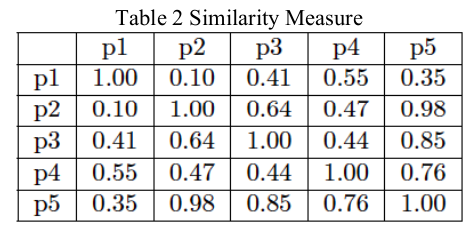
\includegraphics{2.png}
\caption{}
\end{figure}


\subsection*{MIN (Single Link)}

	\begin{table}[H]
	\centering
    \begin{tabular}{|l|r|l|l|l|l|l|r|}
    	\toprule
    	{} &  1 & 2 &      3 & 4 &        5 \\
    	\midrule
    	1 &  1 & 0.1 & 0.41 &    0.55 & 0.35  \\
    	2 &  0.1 & 1 &    0.64 & 0.47 &  0.98 \\
    	3 &  0.41 & 0.64 &    1 & 0.44 &  0.85 \\
    	4 &  0.55 & 0.47 &    0.44 & 1 &  0.76 \\
    	5 &  0.35 & 0.98 &    0.85 & 0.76 &  1 \\
    	\bottomrule
    \end{tabular}
	\end{table}


	\begin{table}[H]
	\centering
	\begin{tabular}{|l|r|l|l|l|l|l|r|}
		\toprule
		{} &  1 2 &      3 & 4 &        5 \\
		\midrule
		12 &  1 & 0.41 &    0.47 & 0.35  \\
		3 &  0.41 & 1 &   0.44 &  0.85 \\
		4 & 0.47 &    0.44 & 1 &  0.76 \\
		5 &  0.35 &   0.85 & 0.76 &  1 \\
		\bottomrule
	\end{tabular}
\end{table}


\begin{table}[H]
	\centering
	\begin{tabular}{|l|r|l|l|l|l|l|r|}
		\toprule
		{} &  125& 3 & 4 \\
		\midrule
		125 &  1 & 0.41 &    0.47 \\
		3 &  0.41 & 1 &   0.44 \\
		4 & 0.47 &  0.44 & 1\\
		\bottomrule
	\end{tabular}
\end{table}


\begin{table}[H]
	\centering
	\begin{tabular}{|l|r|l|l|l|l|l|r|}
		\toprule
		{} &  1253&  4 \\
		\midrule
		1253 &  1 & 0.44  \\
		3 &  0.44 & 1 \\
		\bottomrule
	\end{tabular}
\end{table}

\begin{figure}[H]
	\centering
	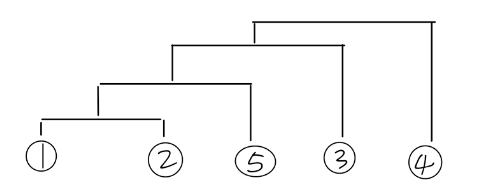
\includegraphics{4.png}
	\caption{}
\end{figure}


\subsection*{MAX (Complete Link)}

\begin{table}[H]
	\centering
	\begin{tabular}{|l|r|l|l|l|l|l|r|}
		\toprule
		{} &  1 & 2 &      3 & 4 &        5 \\
		\midrule
		1 &  1 & 0.1 & 0.41 &    0.55 & 0.35  \\
		2 &  0.1 & 1 &    0.64 & 0.47 &  0.98 \\
		3 &  0.41 & 0.64 &    1 & 0.44 &  0.85 \\
		4 &  0.55 & 0.47 &    0.44 & 1 &  0.76 \\
		5 &  0.35 & 0.98 &    0.85 & 0.76 &  1 \\
		\bottomrule
	\end{tabular}
\end{table}


\begin{table}[H]
	\centering
	\begin{tabular}{|l|r|l|l|l|l|l|r|}
		\toprule
		{} &  25 &1 &      3 & 4 \\
		\midrule
		25 &  1 & 0.1 &    0.64 & 0.47  \\
		1 &  0.1 &   1 & 0.41 &  0.55 \\
		3 &  0.64 & 0.41 &   1 &  0.44 \\
		4 & 0.47 &   0.55 & 0.44 &  1 \\
		\bottomrule
	\end{tabular}
\end{table}


\begin{table}[H]
	\centering
	\begin{tabular}{|l|r|l|l|l|l|l|r|}
		\toprule
		{} &  253 & 1 & 4 \\
		\midrule
		253 &  1 & 0.1 &    0.44 \\
		1 &  0.1 & 1 &   0.55 \\
		4 & 0.44 &  0.55 & 1\\
		\bottomrule
	\end{tabular}
\end{table}


\begin{table}[H]
	\centering
	\begin{tabular}{|l|r|l|l|l|l|l|r|}
		\toprule
		{} &  253&  14 \\
		\midrule
		253 &  1 & 0.1  \\
		14 &  0.1 & 1 \\
		\bottomrule
	\end{tabular}
\end{table}


\begin{figure}[H]
	\centering
	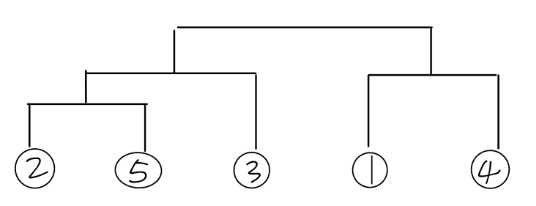
\includegraphics{5.png}
	\caption{}
\end{figure}


    \subsection*{Q3}\label{q3}

\begin{enumerate}
\def\labelenumi{\arabic{enumi}.}
\setcounter{enumi}{2}
\tightlist
\item
  (20\%) Identify possible clusters in the figure below using DBSCAN.
  Please indicate the number of clusters for each case and briefly
  explain your reasoning. Note that darkness or the number of dots in an
  area visually indicates its density.
\end{enumerate}

\begin{figure}[H]
\centering
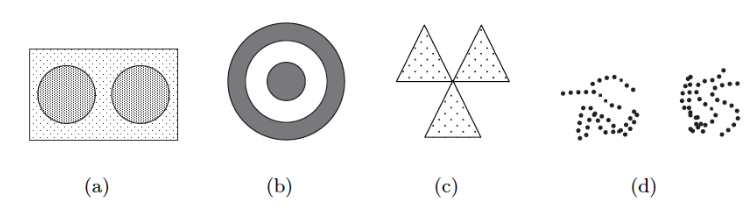
\includegraphics{3.png}
\caption{}
\end{figure}

    \begin{itemize}
\item
  \begin{enumerate}
  \def\labelenumi{\arabic{enumi}.}
  \item
  \end{enumerate}

  \begin{itemize}
  \tightlist
  \item
    Clusters: 2
  \item
    Density-based using DBSCAN
  \item
    reason: The inner points in circle are core points and the exterior
    are noise
  \end{itemize}
\item
  \begin{enumerate}
  \def\labelenumi{\arabic{enumi}.}
  \setcounter{enumi}{1}
  \item
  \end{enumerate}

  \begin{itemize}
  \tightlist
  \item
    Clusters: 2
  \item
    Density-based using DBSCAN
  \item
    reason: The points in inner  circle and outer ring are core points.
  \end{itemize}
\item
  \begin{enumerate}
  \def\labelenumi{\arabic{enumi}.}
  \setcounter{enumi}{2}
  \item
  \end{enumerate}

  \begin{itemize}
  \tightlist
  \item
    Clusters: 3
  \item
    Center-based not using DBSCAN (probably using KMeans)
  \item
    reason: The clustering is partitional clustering with centroids as the mean of points in each individual cluster (in this case, each triangle).
  \end{itemize}
\item
  \begin{enumerate}
  \def\labelenumi{\arabic{enumi}.}
  \setcounter{enumi}{3}
  \item
  \end{enumerate}

  \begin{itemize}
  \tightlist
  \item
    Clusters: 2
  \item
    Contiguity-based using DBSCAN or hierarchal clustering
  \item
    reason: The clustering is contiguity-based, the two clusters are formed because the data points in each cluster are continuous and also the density of the two clusters is higher than the region between them.
  \end{itemize}
\end{itemize}


    % Add a bibliography block to the postdoc
    
    
    
    \end{document}
